\chapter{Theoretische Grundlagen}
\label{cha:Grundlagen}


%%%%%%%%%%%%%%%%%%%%%%%%%%%%%%%%%%%%%%%%%%%%%%%%%%%%%%%%%%
%%%%%%%%%%				HTML					%%%%%%%%%%				
%%%%%%%%%%%%%%%%%%%%%%%%%%%%%%%%%%%%%%%%%%%%%%%%%%%%%%%%%%
\section{HTML}
\label{sec:HTML}
%%%%%%%%%%%%%%%%%%%%%%%%%%%%%%%%%%%%%%%%%%%%%%%%%%%%%%%%%%

Um das Verständnis für die Projekteinführung zu erlangen und die im Kapitel 3 beschriebene Durchführung nachvollziehen zu können, wird in diesem Kapitel zuerst der literarische Bogen von \ac{HTML} über \ac{CSS}, JavaScript und abschließend zu AngularJS gespannt. \ac{HTML} ist, ähnlich wie Latex, eine textbasierte Skriptsprache zur Beschreibung von Websiten. Diese werden von Webbrowsern, wie z.B. Google Chrome, zur Darstellung interpretiert. 

%%%%%%%%%%%%%%%%%%%%%%
\begin{description}
	\item[Aufbau einer HTML Datei]
    \hfill 
    \label{des:Aufbau_HTML}
\end{description}
%%%%%%%%%%%%%%%%%%%%%%
%
\begin{lstlisting}[language=HTML]
<!DOCTYPE html>
<html lang="de">
<head>
    <title>Kiwilabs Rechnungs-WebApp</title>
    <meta name="viewport" content="width=device-width, initial-scale=1">

</head>
<body>
    <h1> Dies ist eine Überschrift </h1>
</body>
\end{lstlisting}

Generell kann das \ac{HTML} Dokument in den sog. \textit{Head} und \textit{Body} unterteilt werden. Solche Abschnitte werden mit einem entsprechenden Tag geöffnet, bzw. geschlossen. Ein Tag ist eine Anweisung in einer spitzen Klammer und liefert dem Browser Informationen über die Struktur des zu darstellenden Dokuments. Der Aufrufer der WebSite sieht nur die Daten, die im Body-Tag beschrieben sind.\cite{html_huberlin}. Ein \textit{<p>-Tag} erzeugt einen Absatz mit Zeilenumbruch, ein <h1, h2, h3, etc.> Tag erzeugt eine Überschrift, wie hier der h1 Tag \bashCommand{<h1> Dies ist eine Überschrift </h1>}, Z.9. 
Der sogenannte \textit{<div>}-Tag wird vor allem benutzt, um mehrere \ac{HTML}-Blöcke zu gruppieren und anschließend mit Hilfe von \ac{CSS} zu formatieren.

\begin{figure}
  \centering
  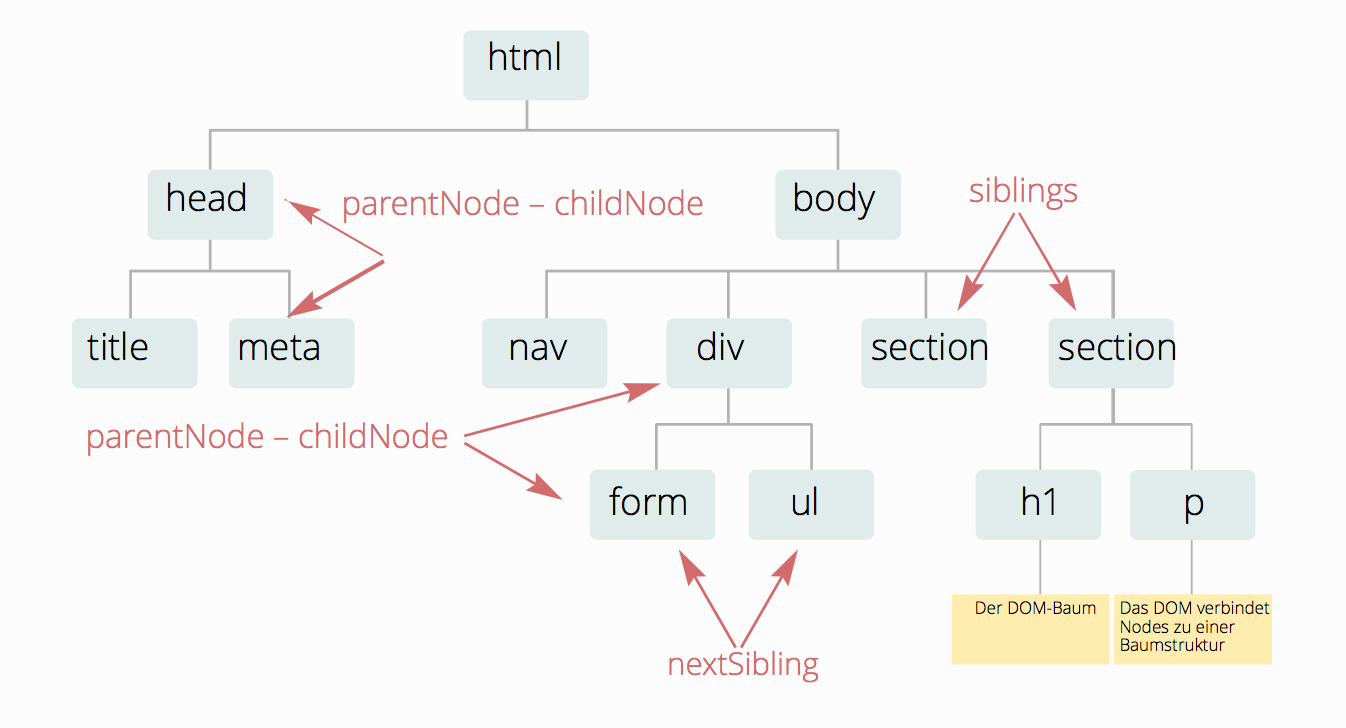
\includegraphics[width=0.7\textwidth]{imports/HTML}
  \caption{Aufbau eines HTML-Dokuments \cite{dom.html}}
\end{figure}









%%%%%%%%%%%%%%%%%%%%%%%%%%%%%%%%%%%%%%%%%%%%%%%%%%%%%%%%%%
%%%%%%%%%%					CSS					%%%%%%%%%%
%%%%%%%%%%%%%%%%%%%%%%%%%%%%%%%%%%%%%%%%%%%%%%%%%%%%%%%%%%
\section{CSS}
\label{sec:CSS}
%%%%%%%%%%%%%%%%%%%%%%%%%%%%%%%%%%%%%%%%%%%%%%%%%%%%%%%%%%

%%%%%%%%%%%%%%%%%%%%%%
\begin{description}
	\item[Die Definition und Bedeutung von CSS]
    \hfill 
    \label{des:Def_CSS}
\end{description}
%%%%%%%%%%%%%%%%%%%%%%
%
Die Seitenbeschreibungssprache \ac{HTML} dient zusammenfassend dem grundsätzlichen Aufbau der Website und definiert somit den Content. Standardmäßg werden allerdings die einzelnen \ac{HTML} Elemente nur untereinander aufgereiht und besitzen nur wenige, von dem Browser vorgegebene Formatierungen. Hier schafft\ac{CSS} Abhilfe, auf das in diesem Abschnitt eingegangen wird. So ist es eine Formatierungs- und Gestaltungssprache, mit der man fähig ist, die zuvor mittels \ac{HTML} erzeugten Elemente gezielt zu platzieren, deren Farbe und Form zu verändern und die aufzubauende Website folglich nach eigenem persönlichem Geschmack zu formatieren. Die Philosophie hierfür ist eine Trennung des Aufbaus der Website in Inhalt (\ac{HTML}) und Gestaltung (\ac{CSS}) \cite{css}.

%%%%%%%%%%%%%%%%%%%%%%
\begin{description}
	\item[Der Aufbau eines Stylesheets - Verwendung der \ac{CSS}-Regeln]
    \hfill
    \label{des:Aufbau_CSS}
\end{description}
%%%%%%%%%%%%%%%%%%%%%%
%
Der Aufbau des Stylesheets erfolgt durch die Festlegung der \ac{CSS} Regeln. Diese definieren jeweils die Formatierung eines \ac{HTML} ELements. So erfolgt der Aufbau durch eine Voranstellung eines Selektors und eines darauf folgenden Deklarators. Ersteres wählt das gewünschte, zu formatierende \ac{HTML} Element aus, zum Beispiel durch die Verwendung eines <p> Tags. Davon gibt zweiteres die Art und Weise an. Diese wird von geschweiften Klammern umgeben und enthält,von einem Doppelpunkt getrennt, zuerst die Eigenschaft und dann den Wert \cite{css-lernen}.

\newpage
%%%%%%%%%%%%%%%%%%%%%%
\begin{description}
	\item[Die diversen Arten der Selektoren - Tags, IDs und Klassen]
    \hfill
	\label{des:Selektoren_CSS}
\end{description}
%%%%%%%%%%%%%%%%%%%%%%
%
Im Folgenden wird die mögliche Verwendung von Selektoren beschrieben. Diese können entweder Tags, IDs oder Klassen sein. \textit{Tag-Selektoren} wählen, wie der Name sagt, alle Tags einer Art aus. Der \textit{ID-Selektor} wird verwendet, um einzelnen \ac{HTML} Elementen Eigenschaften zu zuweisen. Dieser wird durch das Hashtag Symbol begonnen und darauf folgend ist die \textit{HTML-ID}. Die definierten Eigenschaften gelten nun nur für das spezifische Element mit der identischen ID. 
Wenn\ac{HTML} Elemente, die mehrere, bzw. unterschiedliche Tags besitzen, nach gleichem Style formatiert werden sollen, muss auf \textit{Klassen-Selektoren} zurück gegriffen. Diese werden mit einem anfänglichem Punkt und dem Klassennamen definiert. 

\begin{table}
  \centering
  \begin{tabular}{|l|l|} \hline
  Externe Stylesheets    & Definition der Regeln in externer Formatvorlage          \\ \hline
  Inline Styles          & Direktes Festlegen der Regeln in öffnendem Tag der Datei \\ \hline
  Styles im Head Bereich & Definition der Regeln im Kopf Bereich der \ac{HTML} Datei \\ \hline
  \end{tabular}
  \label{tab:Integrationsmöglichkeiten}
  \caption{Integrationsmöglichkeiten von \ac{CSS} in \ac{HTML}}
\end{table}

%%%%%%%%%%%%%%%%%%%%%%
\begin{description}
	\item[Die Verwendung von externen Stylesheets]
    \hfill
    \label{des:Aufbau_CSS}
\end{description}
%%%%%%%%%%%%%%%%%%%%%%
%
Es gibt verschiedene Integrationsmöglichkeiten von \textit{CSS} in die \textit{HTML} Datei. Im Zuge der Arbeit wird allerdings nur auf die in dem Projekt angewandte Möglichkeit der Benutzung von externen Stylesheets eingegangen. Hier wird die Formatierung und Gestaltung in einer externen Datei ausgelagert. Die direkte Verknüpfung erfolgt dann mit einem <link> Tag. Dieses muss immer im Head der \ac{HTML} Datei stehen und verlangt zwei Attribute. Zum einem \textit{rel}, was die Beziehung des verlinkten Dokuments zur \ac{HTML} Datei angibt. Zum Anderen \textit{href}, das die URL zum verlinkten Dokument mitgibt. Der Vorteil der Verwendung von einem externen Stylesheet ist die erhöhte Flexibilität des Websitenstyles und die gesteigerte Effizienz, da diese gestaltungsgebende Datei nach Bedarf leicht ausgetauscht und zudem für mehrere \ac{HTML}-Dateien verwendet werden kann \cite{kaskade}.

\lstinputlisting[language=HTML, firstline=9, lastline=9, firstnumber=9]{src/main.html}



%%%%%%%%%%%%%%%%%%%%%%
\begin{description}
	\item[Die Gestaltung des Seitenlayouts]
	\hfill 
    \label{des:Layout_CSS}
\end{description}
%%%%%%%%%%%%%%%%%%%%%%
%
In \ac{CSS} können \ac{HTML}-Elemente grundsätzlich in zwei Arten unterteilt werden: Block- und Inline Elemente. Erstere sind klar abgegrenzte Bereiche, da sie vor und hinter sich einen Zeilenumbruch bewirken und als rechteckige Boxen dargestellt werden. Deren Breite, Höhe oder Abstand kann man beliebig festlegen. Die Darstellung von dieser Elementart und Zusammenfassung in einem Layout erfolgt über das Box-Modell.(vgl.Abb.2.2) Mit diesem kann das Layout in 4 Bereiche differenziert werden und hilft so zu einem übersichtlichen Seitenlayout Entwurf. 
%
\begin{figure}
  \centering
  
\includegraphics[width=0.7\textwidth]{imports/boxmodell.png}
  \caption{Das Box-Modell \cite{boxmodell}}
\end{figure}
%
Inline Elemente hingegen erzeugen keinen Zeilenumbruch, somit kann man zum Beispiel einzelne Wörter als solche festlegen. Die Maße sind folglich nicht individuell setzbar, sondern automatisch so lang wie das Wort. 










%%%%%%%%%%%%%%%%%%%%%%%%%%%%%%%%%%%%%%%%%%%%%%%%%%%%%%%%%%
%%%%%%%%%%			JavaScript					%%%%%%%%%%
%%%%%%%%%%%%%%%%%%%%%%%%%%%%%%%%%%%%%%%%%%%%%%%%%%%%%%%%%%
\section{JavaScript}
\label{sec:JavaScript}
%%%%%%%%%%%%%%%%%%%%%%%%%%%%%%%%%%%%%%%%%%%%%%%%%%%%%%%%%%

%%%%%%%%%%%%%%%%%%%%%%
\begin{description}
	\item[ Die Intention der Verwendung von Javascript]
    \hfill
    \label{des:Intention_JS}
\end{description}
%%%%%%%%%%%%%%%%%%%%%%
%
Für eine Websitenprogrammierung wird  neben dem Wissen über \ac{CSS} und \ac{HTML} auch ein Repertoire an verfügbarem Javascript Know-How benötigt. JavaScript wirdin eine \ac{HTML} Datei eingebunden und man ist mit Hilfe diesem Werkzeug in der Lage, beliebigen Text in einer schon dargestellten Website zu ändern. Dies ist beispielsweise bei einer immer aktuellen Anzeige der Uhrzeige auf der Website notwendig. Außerdem können dynamische Charakteristika, wie etwa das Öffnen oder Schließen von Optionen/Dateien, durch Javascript gesteuert werden \cite{javascript}.


%%%%%%%%%%%%%%%%%%%%%%
\begin{description}
	\item[Das Einbinden in das \ac{HTML}-Dokument ]
	\hfill
    \label{des:Einbindung_JS}
\end{description}
%%%%%%%%%%%%%%%%%%%%%%
%
Implementiert wird Javascript mit dem Kommando \textit{<Script>} und beendet mit \textit{</script>}, in diesem Bereich können Aufforderungen über die Dynamik der Website definiert werden. Dies kann durch einen direkten Aufruf oder über eine Einbindung einer externen Script Datei geschehen \cite{javascript}.


\newpage
%%%%%%%%%%%%%%%%%%%%%%
\begin{description}
	\item[AngularJS im Rahmen der Anwendung von Javascript]
    \hfill
    \label{des:AngularJS}
\end{description}
%%%%%%%%%%%%%%%%%%%%%%
%
Eine Option für ein JavaScript ist Angular JS. Es ist OpenSource von Google entwickelt worden. Es vereinfacht unter Anderem den Datenaustausch zwischen Frontend und Logik. Deswegen wird im folgenden auf dieses Javascript Webframework eingegangen, da es eine wichtige Rolle für die Umsetzung des Projektes spielt.
Mit AngularJs werden Direktiven, sogenannte \textit{ng-directives} in die \ac{HTML}-Datei eingebunden. Dadurch können Eingaben des Websitenbesuchers übernommen werden. Die Direktive \textit{ng-model} verbindet eine Variable mit dem Frontend. Diese kann eine Eingabe des Nutzers entgegen nehmen oder auf der Website ausgegeben werden. Diese zwei Direktiven sind die grundlegendsten Arten. Auf die in dem Projekt tatsächlich verwendeten Direktiven wird später eingegangen. 
An dieser Stelle ist die Unterscheidung der AngularJS Applikationen in die sogenannten \textit{modules} und \textit{controllers} wichtig. Ersteres definiert die AngularJS Applikation \cite{angularjs}.
\hfill
Beispielcode:

\begin{lstlisting}[language=JavaScript]	
	var applikation = angular.module('myapplikation', []);
\end{lstlisting}

Der \textit{controller} steuert einen Teil der Applikation. In folgendem Beispielcode besitzt er den Namen \textit{myController}. AngularJS ruft den Controller mit einem \textit{scope} Objekt auf. In diesem legt der \textit{controller} zwei Variablen an: \textit{firstName} und \textit{lastName}. 

\begin{lstlisting}[language=JavaScript]	
app.controller('myCtrl', function($scope) {
    $scope.firstName = "Max";
    $scope.lastName = "Muster";
});
\end{lstlisting}

Dies ist das grundlegende Wissen, das für die Durchführung des Projektes benötigt wird. 














